% Chapter 1

\chapter{Introduction} % Main chapter title

\label{ch:intro} % For referencing the chapter elsewhere, use \ref{Chapter1} 

\lhead{1. \emph{Introduction}} % This is for the header on each page - perhaps a shortened title

%----------------------------------------------------------------------------------------

%\section{Welcome and Thank You}

%problem description
In simulation modeling, we seek to capture the behavior of a physical system by describing it in a
\emph{model}, a series
of mathematical equations.  These often take the form of partial differential equations.  These models may be
time- and spacially-dependent, and capture
physics of interest for understanding the system.  A \emph{solver} is then written that can solve the series
of equations and determine \emph{responses}, or quantities of interest, often through numerical evaluations on
computation devices.  A traditional solver accepts a set of inputs and
produces a set of single-valued outputs.  For instance, a solver might solve equations related to the
attenuation of a beam of photons through a material, and the response might be the strength of the beam exiting the
material.  A single evaluation of the solver usually results in a single value, or realization, of the
response.  Figure \ref{fig:model} shows these relationships, and provides an example for nuclear reactor criticality 
calculations.
\begin{figure}[H]
  \centering
  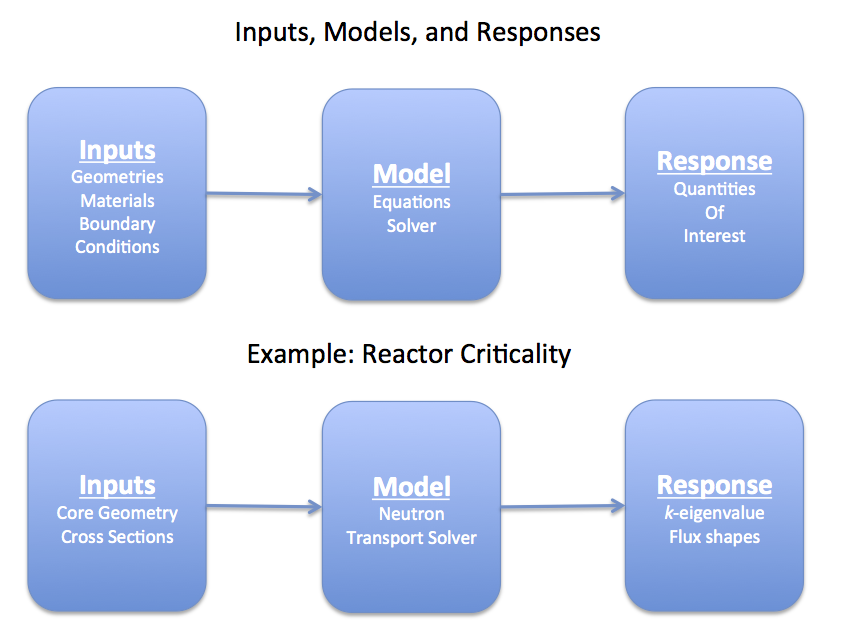
\includegraphics[width=0.7\linewidth]{models}
  \caption{Example Models}
  \label{fig:model}
\end{figure}

This single realization might be misleading, however.  In most systems there is some degree of uncertainty in
the input parameters to the solver.  Some of these uncertainties may be epistemic, or systematic uncertainty
originating with inexact measurements or measurable unknowns.  Other uncertainties might be aleatoric,
intrinsic uncertainty in the system itself, such as probabilistic interactions or random motion.  Taken
together, the input parameter uncertainties exist within a multidimensional probabilistic space.  This
multidimensional probabilistic space is weighted by the probability of realizations occurring in hypervolumes
within the space.  While some
points in that space may be more likely than others, the possible range of values for the response is only
understood when the uncertain input space is considered as a whole and propagated through the model.  We note 
here that while it is possible
that some of the input parameters are correlated in their probabilistic distribution, it is also possible to
decouple them into independent variables (see \ref{sec:KL}).  Throughout this work we will assume the input parameters 
are independent.

%Monte Carlo
One traditional method for exploring the uncertain input space is through random sampling, such as in analog Monte
Carlo sampling.  In this method, a point in the input space is chosen at random based on probability.  This
point represents values for the input parameters to the solver.  The solver is executed with these inputs, and
the responses are collected.  Then, another point in the input space is chosen at random.  This process continues
until the properties of the response are well understood.

There are some beneficial properties to random sampling approaches like Monte Carlo.  
Significantly, they are unintrusive:
 there is no need to modify the solver in order to use these methods.  This allows a framework of
algorithms to be developed which know only the input space and response of a solver, but need no further knowledge
about its operation.  Unintrusive methods are desirable because the uncertainty quantification algorithms can
be developed and maintained separately from the solver, such as frameworks like \raven{} \cite{raven}.

Monte Carlo (MC) and similar sampling strategies are relatively slow to converge the response surface.  The
response surface is the space of all possible outcomes for the model given the uncertainty in the inputs,
weighted by the probability of that outcome occurring. This surface is difficult to converge accurately in MC.  For
example, in order to reduce the standard error of the mean of the response by a factor
of two using MC, it is necessary to evaluate the model four times more often.  If a solver is sufficiently computationally
inexpensive, obtaining additional evaluations is not a large concern; however, for lengthy and expensive
solvers such as those found commonly in nuclear engineering applications,
it may not be practical to obtain sufficient realizations to obtain a clear response surface.
In this work MC is used as a benchmark methodology; if other methods converge on moments of the responses
more quickly and consistently than MC, we consider them ``better'' for our purposes.

The first advanced uncertainty quantification  method we consider is Stochastic Collocation for generalized Polynomial
Chaos (SCgPC) \cite{sparseSC,sparse1,sparse2,xiu}, wherein deterministic collocation points 
are used to develop a polynomial-interpolated surrogate model
of the response as a function of the inputs.  This method algorithmically expands the solver as the sum of
orthogonal multidimensional polynomials with scalar coefficients.  The scalar coefficients are obtained by
numerical integration using multidimensional collocation (quadrature) points.  The chief distinction between
SCgPC and MC methods is that SCgPC is deterministic, in that the realizations required from the
solver are predetermined instead of randomly sampled.
Like Monte Carlo, SCgPC is unintrusive
and performs well without any need to access the internal operations of the solver.  This behavior is desirable for
construction of black-box approach algorithms for uncertainty quantification.  Other intrusive methods such as
Stochastic Galerkin exist \cite{galerkin}, but require solver modification to operate.  This makes them
solver-dependent and undesirable for an independent uncertainty quantification framework.

The other methods we present here expand on standard
SCgPC.  First, we explore non-tensor-product methods for determining the set of polynomial bases to
use in the expansion.  Because a tensor product grows exponentially with increasing dimensionality of the input
space, we combat this curse of dimensionality using
alternative polynomial set construction methods \cite{hctd}.
These polynomial bases will then be used to construct Smolyak-like sparse grids \cite{smolyak} to provide collocation
points that are used to calculate the coefficients in the polynomial expansion.  Further, we consider
anisotropic sparse grids,
allowing higher-order polynomials for particular input parameters.  We also consider methods for
obtaining weights that determine the level of anisotropic preference to give parameters, and explore the effects of a
variety of anisotropic choices.

The second method group we consider is High-Dimensional Model Representation (HDMR), sometimes also referred
to as high-density model reduction, which is based on Sobol
decomposition \cite{hdmr}.  This method is useful both for developing sensitivities of the quantity of
interest with respect to subsets
of the input space, as well as constructing a reduced-order representation of the model itself.  We demonstrate the strength of HDMR
as a method to inform anisotropic sensitivity weights for SCgPC.

Finally, we consider adaptive algorithms to construct both SCgPC and HDMR expansions using second-moment
convergence criteria.  We analyze these for potential efficiencies and shortcomings.  We also propose future
work to further improve the adaptive methods.

% expensive solvers need low-sample UQ
This work is premised on the idea that solvers are often computationally expensive, requiring many hours per
evaluation, and that
computational resource availability requires an analyst perform as few evaluations as possible.  As such, 
we consider several methodologies for quantifying the uncertainty in expensive solver
calculations.  In order to demonstrate the range of operation for these methods, we apply them first on
several analytic problems, such as polynomial evaluations.  These models have a high
degree of regularity, and their analyticity provides for straightforward benchmarking.  Through gradual
increasing complexity, we investigate the behavior of the advanced UQ methods (SCgPC and HDMR) in comparison to MC.

However, the problems facing nuclear engineering analysts today are rarely analytic and have simple forms.  As
a result, we also demonstrate three applications of SCgPC and HDMR to engineering-scale applications.  The
first is a single-physics neutronics benchmark problem that models a small reactor core.  
While the responses of this model have no simple
analytic form, the underlying physics are well-understood and provide for good analysis.
The second
engineering-scale application is a multiphysics problem modeling nuclear fuel through burnup depletion.  This
model couples neutronics and fuels performance nonlinearly, where neutronics provides flux shapes that
determine power shapes for fuels performance, and fuels performance provides temperature feedbacks to the
nuclear cross sections.
Finally, we demonstrate how HDMR and SCgPC can be used to analyze a time-dependent fuels performance problem
in which a fuel rod undergoes several changes in power level over a long period of irradiation.  Instead of
converging moments of responses, this last analysis concerns using changing sensitivity parameters to detect
changes in dominant physics during a transient problem.

We implement all the advanced UQ methods in Idaho National Laboratory's \raven{} \cite{raven}
uncertainty quantification framework. \raven{} is a Python-written framework that non-intrusively provides
tools for analysts to quantify the uncertainty in their simulations with minimal development.  To demonstrate
the application of the methods developed, we apply \raven{} to complex non-linear solvers.
To simulate neutronics and fuels performance, we use \rattlesnake{} \cite{rattlesnake} and 
\bison{} \cite{bison,mammoth} production codes respectively.
Both of these codes are developed in and based on the \moose{} \cite{moose} environment.

%outline chapters
The remainder of this work will proceed as follows:

\begin{itemize}
  \item Chapter 2: We consider SCgPC as an uncertainty
    quantification method in comparison to Monte Carlo.  We discuss implementation of several polynomial
    expansion types as well as both isotropic and anisotropic approaches.  We additionally consider an
    adaptive scheme for the polynomial expansion, and offer some improvements on existing efforts in
    adaptivity.
  \item Chapter 3: We present the performance of SCgPC
    expansion methods as applied to a variety of analytic models.  We analyze a set of increasingly-complex
    models and contrast collocation methods on models of varying dimensionality.  We draw some conclusions
    based on performance to determine when SCgPC is a viable choice over Monte Carlo sampling.
  \item Chapter 4: Expanding on SCgPC, we further consider
    HDMR, achieved through Sobol decomposition.  We apply generalized polynomial
    chaos expansions to the subspace terms in the HDMR expansion, and demonstrate
    synergies with the two expansions.  Further, we present a combined adaptive scheme for the two expansion
    methods and offer improvements on existing adaptive methods.
  \item Chapter 5: We add the performance of HDMR to the previous analyses of analytic
    models, and consider the merits and shortcomings of several truncation orders of HDMR 
    eduction.  We also consider the adaptive HDMR method when compared with the SCgPC
    methods.
  \item Chapter 6: We apply the uncertainty quantification techniques described in this work to a
    single-physics neutronics benchmark problem.  We consider the efficiencies and limitations of both
    SCgPC and HDMR as uncertainty
    quantification tools for this model, and discuss some findings due to this non-analytic model. 
  \item Chapter 7: We further apply the advanced uncertainty quantification techniques to a multiphysics
    engineering-scale problem coupling fuels performance to neutronics.  We consider the efficiency of select
    methods discussed, and limitations discovered from these coupled codes.
  \item Chapter 8: We consider application of low-order HDMR to a time-dependent fuels
    performance benchmark.  We present the development of Sobol sensitivity coefficients between responses of
    interest and uncertain input parameters over a time-dependent problem.  Further, we demonstrate how these
    sensitivities can yield additional comprehension of the underlying physical models.  We discuss briefly
    the limitations discovered as a result of performing this analysis.
  \item Chapter 9: We summarize the efforts of this paper and offer conclusions, including the types of models
    for which the uncertainty quantification techniques are efficient, when they can be expected to be
    inefficient, and when they will not work altogether.  We also suggest some future work efforts that are logical
    progressive steps from the work performed here.
\end{itemize}
%----------------------------------------------------------------------------------------
